% SC1005 --- Chapter 6: Registers and Counters (0->100)
\chapter{Registers and Counters}
\label{ch:registers}

\begin{quote}
\emph{``Registers hold; counters count; shift registers do both.''}
Built from flip-flops, these are the first useful sequential subsystems---data
storage, sequencing, and serial--parallel conversion in one chapter.
\end{quote}

\noindent\fbox{\parbox{\dimexpr\linewidth-2\fboxsep-2\fboxrule}{%
\textbf{From zero: flip-flops $\to$ systems.} We assume D/JK flip-flops (Ch.~\ref{ch:sequential})
and FSM ideas (Ch.~\ref{ch:fsm}). Each circuit is derived from ``what next-state do we want?''}}
\vspace{0.4em}

\section*{Learning Outcomes}
After this chapter you will be able to:
\begin{enumerate}[label=(L\arabic*)]
    \item build parallel registers with load and clear controls;
    \item explain shift registers and serial/parallel conversion;
    \item design ripple and synchronous counters (binary, decade, up/down);
    \item analyse counter timing, modulus, and self-correcting design;
    \item distinguish ring and Johnson counters and their decoded outputs.
\end{enumerate}

% ============================================================
\section{Registers: Parallel Storage}
\label{sec:registers}
A $n$-bit \emph{register} is $n$ D flip-flops sharing a clock and control signals.
Simplest: $n$ DFFs with common CLK---data $D_{n-1}\dots D_0$ latched on the rising edge.
Additions: \emph{asynchronous clear} ($\bar{CLR}$ forces $0$), \emph{load enable} ($LD$: when $0$, hold; when $1$, load), and tri-state outputs for bus connection.

\begin{figure}[h]
\centering
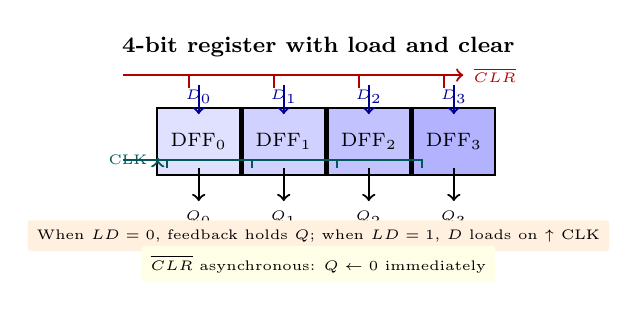
\begin{tikzpicture}[scale=0.80,every node/.style={font=\scriptsize}]
\node[font=\footnotesize\bfseries] at (2.6,2.35) {4-bit register with load and clear};
\foreach \i in {0,1,2,3} {
  \pgfmathsetmacro{\x}{\i*1.35}
  \node[draw,thick,fill=blue!\the\numexpr 12+\i*6\relax,minimum width=1.05cm,minimum height=0.85cm] at (\x+0.7,0.85) {DFF$_{\i}$};
  \draw[->,thick,blue!60!black] (\x+0.7,1.75)--(\x+0.7,1.28) node[above,font=\tiny] {$D_{\i}$};
  \draw[->,thick] (\x+0.7,0.42)--(\x+0.7,-0.1) node[below,font=\tiny] {$Q_{\i}$};
}
% shared clock and controls
\draw[->,thick,teal!70!black] (-0.5,0.55)--(0.05,0.55) node[left,font=\tiny] {CLK} -- (0.05,0.55);
\foreach \i in {0,1,2,3} { \pgfmathsetmacro{\x}{\i*1.35} \draw[thick,teal!70!black] (0.05,0.55)--(\x+0.2,0.55)--(\x+0.2,0.42); }
\draw[->,thick,red!70!black] (-0.5,1.9)--(4.9,1.9) node[right,font=\tiny] {$\overline{CLR}$};
\foreach \i in {0,1,2,3} { \pgfmathsetmacro{\x}{\i*1.35} \draw[thick,red!70!black] (\x+0.55,1.9)--(\x+0.55,1.70); }
% MUX for load
\node[font=\tiny,fill=orange!12,rounded corners=1pt] at (2.6,-0.65) {When $LD=0$, feedback holds $Q$; when $LD=1$, $D$ loads on $\uparrow$ CLK};
\node[font=\tiny,fill=yellow!10,rounded corners=1pt] at (2.6,-1.1) {$\overline{CLR}$ asynchronous: $Q\leftarrow0$ immediately};
\end{tikzpicture}
\caption{Four D flip-flops with common clock, asynchronous clear, and load-hold MUX (conceptually $D_{\text{eff}}=LD\cdot D+\overline{LD}\cdot Q$).}
\label{fig:register}
\end{figure}

Timing is identical to a single DFF: setup/hold on $D$ relative to CLK, $t_{cq}$ to $Q$.
Registers are the state elements of every FSM and data-path.

\section{Shift Registers}
\label{sec:shift}
Connect $Q_i$ to $D_{i+1}$ and data ripples one position per clock---a \emph{shift register}.
Variants: SISO, SIPO, PISO, PIPO (serial/parallel in/out). Add a MUX per stage for \emph{parallel load} vs.\ shift mode,
and a $SI$ (serial in) pin on the first stage.

Applications: serial--parallel conversion (UART), delay lines, sequence generators, and multiplication/division by $2$
(shift left/right).

\begin{figure}[h]
\centering
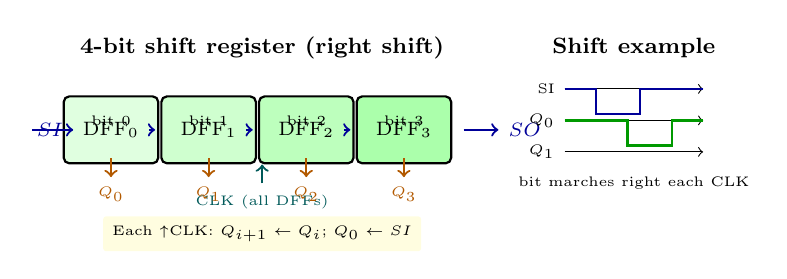
\begin{tikzpicture}[scale=0.80,every node/.style={font=\scriptsize}]
\node[font=\footnotesize\bfseries] at (3.2,2.0) {4-bit shift register (right shift)};
\foreach \i in {0,1,2,3} {
  \pgfmathsetmacro{\x}{\i*1.55}
  \node[draw,thick,fill=green!\the\numexpr 12+\i*7\relax,minimum width=1.20cm,minimum height=0.85cm,rounded corners=2pt] at (\x+0.8,0.7) {DFF$_{\i}$};
  \node[font=\tiny] at (\x+0.8,0.85) {bit \i};
}
\foreach \i in {0,1,2} {
  \pgfmathsetmacro{\x}{\i*1.55}
  \draw[->,thick,blue!60!black] (\x+1.40,0.7)--(\x+1.50,0.7);
}
\draw[->,thick,blue!60!black] (-0.45,0.7)--(0.20,0.7) node[left] {$SI$};
\draw[->,thick,blue!60!black] (6.40,0.7)--(6.95,0.7) node[right] {$SO$};
% clock
\draw[->,thick,teal!70!black] (3.2,-0.15)--(3.2,0.15);
\node[font=\tiny,teal!70!black] at (3.2,-0.45) {CLK (all DFFs)};
% parallel out arrows
\foreach \i in {0,1,2,3} { \pgfmathsetmacro{\x}{\i*1.55} \draw[->,thick,orange!70!black] (\x+0.8,0.25)--(\x+0.8,-0.05) node[below,font=\tiny] {$Q_{\i}$}; }
\node[font=\tiny,fill=yellow!12,rounded corners=1pt] at (3.2,-0.95) {Each $\uparrow$CLK: $Q_{i+1}\leftarrow Q_i$; $Q_0\leftarrow SI$};
% Waveform mini
\begin{scope}[xshift=8.0cm]
\node[font=\footnotesize\bfseries] at (1.1,2.0) {Shift example};
\foreach \y/\lbl in {1.35/SI,0.85/$Q_0$,0.35/$Q_1$} {
  \draw[->,thin] (0,\y)--(2.2,\y);
  \node[font=\tiny,left] at (0,\y) {\lbl};
}
\draw[thick,blue!60!black] (0,1.35)--(0.5,1.35)--(0.5,0.95)--(1.2,0.95)--(1.2,1.35)--(2.2,1.35);
\draw[thick,green!60!black] (0,0.85)--(1.0,0.85)--(1.0,0.45)--(1.7,0.45)--(1.7,0.85)--(2.2,0.85);
\node[font=\tiny] at (1.1,-0.15) {bit marches right each CLK};
\end{scope}
\end{tikzpicture}
\caption{Shift register: cascade of DFFs. Serial input enters at the left; parallel outputs tap each stage. Universal shift register adds MUX per stage for load/shift/hold.}
\label{fig:shift-reg}
\end{figure}

\section{Counters}
\label{sec:counters}
A \emph{counter} cycles through a sequence of states, usually binary counting. Modulus $m$ = number of distinct states.

\paragraph{Ripple (asynchronous) counter.} Chain T flip-flops with $Q_i$ clocking stage $i+1$.
Simple, but delay accumulates and intermediate glitches appear---unsuitable for synchronous decoding.
Mod-$2^n$ from $n$ bits; mod-$m$ ($m\neq2^n$) needs reset logic when $m$ reached.

\paragraph{Synchronous counter.} All flip-flops share CLK and toggle logic is combinational:
$T_0=1$, $T_1=Q_0$, $T_2=Q_1Q_0$, $\dots$, $T_i=\land_{j<i}Q_j$. All bits update simultaneously---faster,
no glitch, at the cost of AND gates.

\begin{figure}[h]
\centering
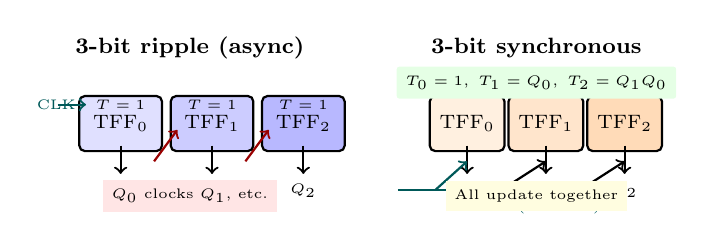
\begin{tikzpicture}[scale=0.80,every node/.style={font=\scriptsize}]
% Ripple 3-bit
\node[font=\footnotesize\bfseries] at (1.8,2.35) {3-bit ripple (async)};
\foreach \i in {0,1,2} {
  \pgfmathsetmacro{\x}{\i*1.45}
  \node[draw,thick,fill=blue!\the\numexpr 12+\i*8\relax,minimum width=1.05cm,minimum height=0.7cm,rounded corners=2pt] at (\x+0.7,1.15) {TFF$_{\i}$};
  \node[font=\tiny] at (\x+0.7,1.45) {$T=1$};
  \draw[->,thick] (\x+0.7,0.80)--(\x+0.7,0.35) node[below,font=\tiny] {$Q_{\i}$};
}
\draw[->,thick,teal!70!black] (-0.3,1.45)--(0.15,1.45) node[left,font=\tiny] {CLK};
\draw[->,thick,red!60!black] (1.23,0.55)--(1.60,1.05); \draw[->,thick,red!60!black] (2.68,0.55)--(3.05,1.05);
\node[font=\tiny,fill=red!10] at (1.8,0.0) {$Q_0$ clocks $Q_1$, etc.};
% Synchronous 3-bit
\begin{scope}[xshift=5.5cm]
\node[font=\footnotesize\bfseries] at (1.8,2.35) {3-bit synchronous};
\foreach \i in {0,1,2} {
  \pgfmathsetmacro{\x}{\i*1.25}
  \node[draw,thick,fill=orange!\the\numexpr 12+\i*8\relax,minimum width=0.95cm,minimum height=0.7cm,rounded corners=2pt] at (\x+0.7,1.15) {TFF$_{\i}$};
  \draw[->,thick] (\x+0.7,0.80)--(\x+0.7,0.35) node[below,font=\tiny] {$Q_{\i}$};
}
\draw[->,thick,teal!70!black] (0.2,0.10)--(0.70,0.55); \draw[->,thick] (1.25,0.10)--(1.95,0.55); \draw[->,thick] (2.50,0.10)--(3.20,0.55);
\node[font=\tiny,fill=green!10,rounded corners=1pt] at (1.8,1.80) {$T_0=1,\;T_1=Q_0,\;T_2=Q_1Q_0$};
\draw[->,thick,teal!70!black] (-0.4,0.10)--(1.8,0.10) node[below,font=\tiny] {CLK (common)};
\node[font=\tiny,fill=yellow!12] at (1.8,0.0) {All update together};
\end{scope}
\end{tikzpicture}
\caption{Ripple vs.\ synchronous 3-bit binary counter. Ripple uses the previous $Q$ as clock (red); synchronous shares CLK and gates the $T$ inputs.}
\label{fig:counters}
\end{figure}

\paragraph{Up/down and decade.} Add a direction bit to select increment vs.\ decrement.
Decade ($0$--$9$) and other non-power-of-two moduli decode terminal count and synchronously reset or use
natural BCD behaviour (e.g.\ 74LS90).

\paragraph{Ring and Johnson.} \emph{Ring}: shift register with $Q_{n-1}$ fed back to $D_0$---one hot circulates ($n$ states, simple decode).
\emph{Johnson (twisted ring)}: feed $\bar Q_{n-1}$ back---$2n$ states with Gray-like adjacency, decoded by 2-literal ANDs.


\section{Counter Modulus, Self-Correction, and Timing}
Modulus $m$ need not be a power of two. For synchronous mod-$m$ ($m<2^n$), decode terminal count $m-1$ and synchronously
load $0$ (or use natural truncated sequence with don't-cares for $m$--$2^n-1$ to minimize logic). Asynchronous reset for mod-$m$
creates a short glitch state (e.g.\ $101\to000$ via $101$ spike)---use synchronous reset in clocked systems.

\emph{Self-correction:} every unused state must eventually enter the valid cycle. Verify by tracing next-state from each unused code;
if a lock-up cycle exists, add logic to break it (usually force to $0$ on next clock). Ring/Johnson counters are inherently
self-correcting only if designed with correction gates (e.g.\ start-up reset).
\begin{example}[Mod-10 decade]
BCD decade $0$--$9$ from 4 bits: states $1010$--$1111$ are don't-cares. K-maps for next-state treat them as $\times$,
yielding simpler logic than a full 16-state map. Add synchronous clear when $1001\to0000$ to close the cycle.
\end{example}

% ============================================================

% ============================================================
\section{Chapter Notes}
Counters and shift registers were the first MSI building blocks (7495, 74193, 74164).
Pipelined data-paths still use registers as pipeline boundaries; Johnson counters appear in stepper-motor drivers.

% ============================================================
\section{Applications: From Counters to Timers}
Counters plus registers build timers, frequency dividers, and UART baud generators. A down-counter loaded with $N$ and counting to $0$
produces a pulse every $N+1$ clocks (programmable period). A prescaler (power-of-two divider) followed by a programmable counter
covers wide timing ranges with modest bit-width. In displays, a BCD counter plus 7-segment decoder drives each digit, multiplexed
at $\sim1$\,kHz so persistence of vision shows a stable number.

% ============================================================

\paragraph{Shift-register applications.} Beyond storage, shift registers implement \emph{sequence generators}
(LFSR with XOR feedback gives maximal $2^n-1$ pseudo-random sequence), \emph{CRC} computation (polynomial division
via shifted XOR), and \emph{serial protocols} (SPI/I$^2$C shift data on SCLK). The universal shift register's four
modes (hold, shift-left, shift-right, parallel load) are selected by two mode bits---one chip, many uses.

\section{Exercises}
\label{sec:ch06-exercises}
\begin{enumerate}[label=E6.\arabic*, leftmargin=*, itemsep=0.8em]
    \item \textbf{Register timing.} A 4-bit register uses DFFs with $t_{su}=15$\,ns, $t_{cq}=20$\,ns. What is max CLK frequency? What changes with a load MUX adding 8\,ns before $D$?
    \item \textbf{Shift modes.} Draw a 4-bit universal shift register stage with MUX selecting hold/shift-left/shift-right/parallel-load. Give the $S_1S_0$ table.
    \item \textbf{Synchronous design.} Design a mod-6 synchronous binary counter (0--5) using T flip-flops. Derive $T_2T_1T_0$ via K-maps and handle states 6,7.
    \item \textbf{Ripple glitch.} Show a 3-bit ripple counter glitch when $011\to100$: list transient binary values and explain why synchronous avoids them.
    \item \textbf{Johnson decode.} For a 4-bit Johnson counter, list its $8$ states and give minimal decode for each state using 2-input gates.
\end{enumerate}
% End of Chapter 6
